% !TeX root = ../documento.tex
\chapter{Resultados e discussão}
\label{chap:resultados-final}

Este capítulo apresenta os resultados de simulação e de bancada obtidos no desenvolvimento do controle digital de um módulo hidráulico de frenagem. Primeiro, são discutidos o comportamento do modelo hidráulico e o desempenho do LQI em simulação; em seguida, apresentam-se a plataforma eletrônica, a transição da configuração inicial com bomba centrífuga para o LAC e os ensaios experimentais. Essa organização distingue as evidências computacionais dos resultados medidos no conjunto físico.

Nas simulações, a pressão hidráulica é a variável utilizada para avaliar o seguimento de referência pelo LQI. Na bancada, o controlador LQI foi aplicado ao posicionamento do atuador linear de êmbolo (LAC), e a pressão resultante foi monitorada para avaliar a resposta hidráulica. A posição do LAC determina o volume deslocado e, em conjunto com a complacência do circuito, influencia a pressão gerada. Portanto, os ensaios físicos validam a execução do LQI no controle de posição e caracterizam a pressão produzida, sem serem interpretados como controle direto da pressão medida.


\section{Simulação do modelo hidráulico em malha aberta}
\label{sec:resultado-final-malha-aberta}

Antes da avaliação do controlador, foi realizado um ensaio integrado em malha aberta no modelo hidráulico de duas pressões. O procedimento foi dividido em pressurização, retenção e alívio. Na primeira fase, a bomba foi acionada com $\omega_p>0$, a válvula de entrada foi comandada para abrir e a válvula de saída permaneceu fechada. Na retenção, a bomba foi desligada e os caminhos de entrada e saída foram fechados. No alívio, a entrada foi fechada e a saída foi aberta.

\begin{figure}[htbp]
    \centering
    \includegraphics[width=0.90\textwidth]{figuras/artigo_ensaio_malha_aberta_integrado_real}
    \caption{Ensaio integrado em malha aberta do modelo hidráulico 2P, com as fases de pressurização, retenção e alívio.}
    \label{fig:resultado-final-malha-aberta}
\end{figure}

O resultado reproduziu a causalidade esperada do circuito. Durante a pressurização, a pressão de suprimento aumentou e transferiu vazão para o volume da roda. Quando os comandos foram removidos, a pressão permaneceu aproximadamente constante, sem geração de pressão causada apenas pela retenção. Na fase de alívio, a abertura da saída produziu a redução de $P_w$. Esse ensaio não constitui uma validação quantitativa da unidade física; ele verifica a coerência do modelo antes da síntese e da avaliação do controlador.

\section{Seguimento de referência em malha fechada}
\label{sec:resultado-final-malha-fechada}

O controlador LQI com observador de Luenberger foi avaliado na planta hidráulica não linear. A síntese baseou-se em uma linearização local, e a avaliação foi realizada no modelo não linear. Essa abordagem permitiu analisar a influência das saturações, da dependência das vazões em relação ao diferencial de pressão e das diferenças entre as dinâmicas de pressurização e alívio.

\begin{figure}[htbp]
    \centering
    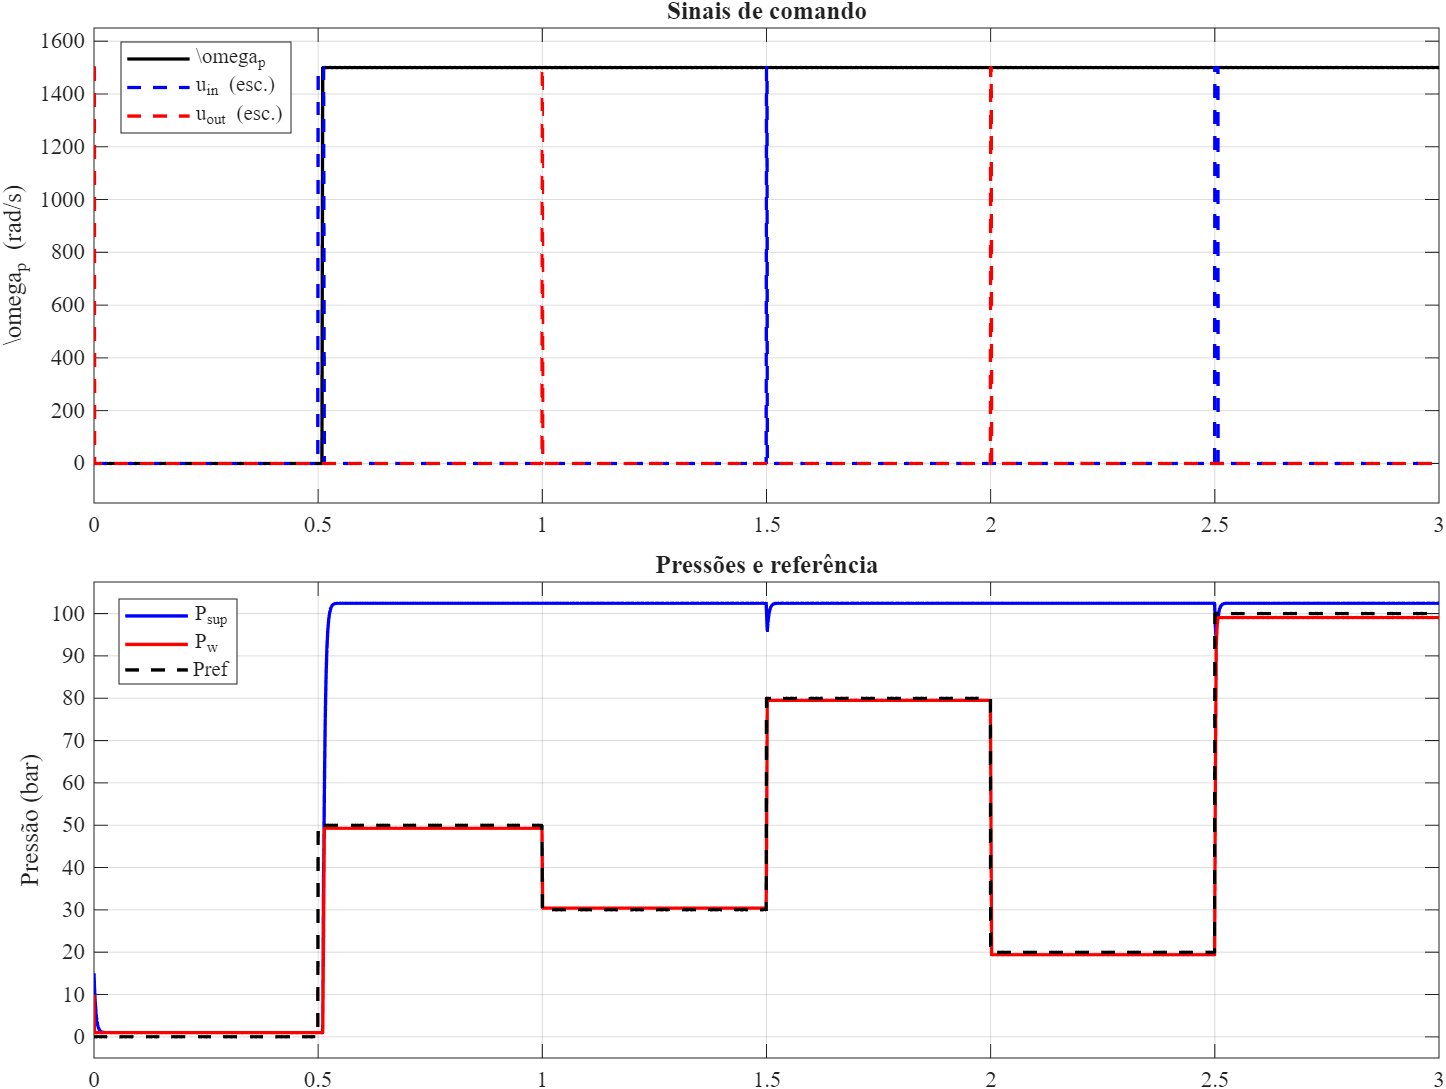
\includegraphics[width=0.92\textwidth]{figuras/simulacao_comandos_e_pressao.png}
    \caption{Comandos e pressão obtidos na simulação em malha fechada com o controlador LQI e o observador de Luenberger.}
    \label{fig:resultado-final-comandos-pressao}
\end{figure}

A resposta simulada acompanhou o perfil de referência em patamares e respeitou as restrições de comando adotadas para a bomba e para as válvulas. O erro não foi uniforme ao longo da trajetória. O maior desvio ocorreu no degrau de $0$ para $50$ bar, enquanto os patamares intermediários apresentaram acomodação mais regular.

\begin{table}[htbp]
    \centering
    \caption{Métricas do cenário nominal de simulação em malha fechada.}
    \label{tab:resultado-final-metricas-nominal}
    \begin{tabular}{l l}
        \toprule
        Indicador & Resultado observado \\
        \midrule
        Erro RMS global & $3{,}68$ bar \\
        Maior RMSE por degrau & $7{,}60$ bar, no trecho $0\rightarrow50$ bar \\
        Sobressinal & Entre $1{,}77\%$ e $7{,}26\%$ \\
        Tempo de subida & Da ordem de milissegundos \\
        Tempo de acomodação & Da ordem de poucos décimos de segundo nos patamares centrais \\
        Esforço de atuação & Maior nas transições de maior amplitude \\
        \bottomrule
    \end{tabular}
    \Fonte{O autor, a partir dos ensaios de simulação.}
\end{table}

\begin{figure}[htbp]
    \centering
    \includegraphics[width=0.92\textwidth]{figuras/artigo_item01_metricas_tracking}
    \caption{Seguimento por degraus e erro de acompanhamento na simulação.}
    \label{fig:resultado-final-metricas-tracking}
\end{figure}

\begin{figure}[htbp]
    \centering
    \includegraphics[width=0.92\textwidth]{figuras/artigo_item01_metricas_desempenho}
    \caption{Métricas de desempenho globais e por degrau.}
    \label{fig:resultado-final-metricas-desempenho}
\end{figure}

As curvas de $\mathrm{d}P_w/\mathrm{d}t$ mostram que os maiores gradientes de pressão coincidem com os períodos de maior atuação. A assimetria entre subida e descida decorre dos caminhos hidráulicos distintos e não deve ser atribuída exclusivamente ao controlador. A análise espectral do regime permanente também permite distinguir ondulações associadas à discretização e à comutação de desvios lentos de rastreamento.

\begin{figure}[htbp]
    \centering
    \includegraphics[width=0.92\textwidth]{figuras/artigo_item02_dpdt_saturacao}
    \caption{Taxa de variação da pressão e atuação próxima aos limites de comando.}
    \label{fig:resultado-final-dpdt}
\end{figure}

\begin{figure}[htbp]
    \centering
    \includegraphics[width=0.92\textwidth]{figuras/artigo_item03_assimetria_subida_descida}
    \caption{Assimetria entre os transientes de pressurização e de alívio.}
    \label{fig:resultado-final-assimetria}
\end{figure}

\begin{figure}[htbp]
    \centering
    \includegraphics[width=0.92\textwidth]{figuras/artigo_item04_ripple_fft}
    \caption{Ondulação em regime permanente no domínio do tempo e da frequência.}
    \label{fig:resultado-final-ripple}
\end{figure}

\section{Robustez, ruído e transições de referência}
\label{sec:resultado-final-robustez}

Foi realizada uma varredura paramétrica para verificar a sensibilidade do desempenho a variações de parâmetros físicos em torno do caso nominal. A mesma lei de controle foi mantida durante os ensaios. Dentro da faixa analisada, observou-se degradação moderada das métricas, sem perda abrupta de seguimento. Esse resultado deve ser entendido como uma avaliação local de robustez por simulação, e não como uma garantia para qualquer variação de parâmetros.

\begin{figure}[htbp]
    \centering
    \includegraphics[width=0.92\textwidth]{figuras/artigo_item06_sensibilidade_parametrica}
    \caption{Sensibilidade das métricas de erro e esforço às variações paramétricas.}
    \label{fig:resultado-final-sensibilidade}
\end{figure}

A variação dos pesos do LQI evidenciou um compromisso entre erro de seguimento e esforço de atuação. A redução do erro pode aumentar a atividade de controle, a ocorrência de saturação e a comutação das válvulas. Com ruído aditivo na medição utilizada pelo observador, o erro RMS e o esforço RMS cresceram de forma gradual na faixa simulada, sem instabilidade abrupta.

\begin{figure}[htbp]
    \centering
    \includegraphics[width=0.92\textwidth]{figuras/artigo_item09_tradeoff_erro_esforco}
    \caption{Compromisso entre erro de seguimento e esforço de atuação para diferentes ponderações do LQI.}
    \label{fig:resultado-final-tradeoff}
\end{figure}

\begin{figure}[htbp]
    \centering
    \includegraphics[width=0.92\textwidth]{figuras/artigo_item10_robustez_ruido}
    \caption{Variação das métricas com o nível de ruído de medição.}
    \label{fig:resultado-final-ruido}
\end{figure}

\section{Plataforma eletrônica e preparação dos ensaios}
\label{sec:resultado-final-plataforma}

Foi desenvolvida uma placa eletrônica para integração com o microcontrolador AURIX TC375 e execução embarcada do controle. Foram produzidas cinco placas: duas receberam todos os componentes disponíveis e três permaneceram sem o driver SB0410. A placa e a arquitetura funcional são apresentadas nas Figuras~\ref{fig:resultado-final-placa} e~\ref{fig:resultado-final-arquitetura}.

\begin{figure}[htbp]
    \centering
    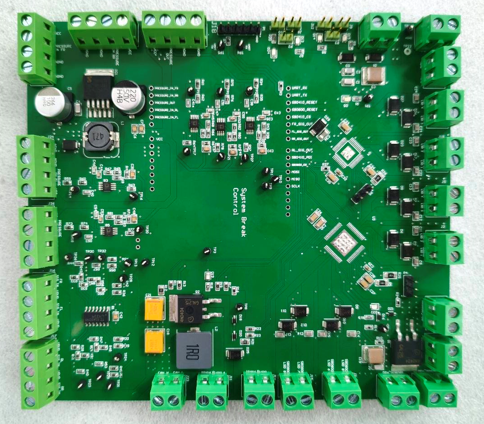
\includegraphics[width=0.82\textwidth]{figuras/imagem_placa_montada.png}
    \caption{Placa eletrônica desenvolvida para a integração com o conjunto de frenagem.}
    \label{fig:resultado-final-placa}
\end{figure}

\begin{figure}[htbp]
    \centering
    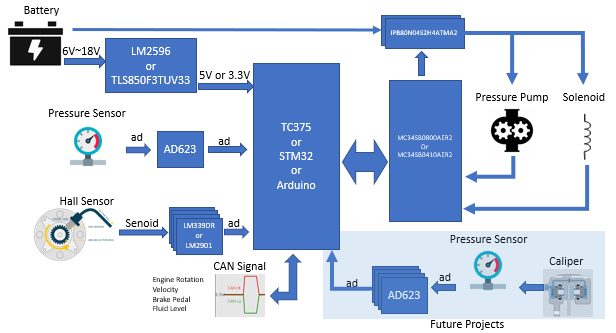
\includegraphics[width=0.92\textwidth]{figuras/arquitetura-funcional-do-sistema-de-controle-de-freio.png}
    \caption{Arquitetura funcional de integração entre controle, aquisição e acionamento.}
    \label{fig:resultado-final-arquitetura}
\end{figure}

Durante a fase de integração física, verificou-se que a tentativa de executar o laço de controle em tempo real fechado diretamente pelo MATLAB/Simulink conectado à bancada via interface USB revelou-se tecnicamente inviável. A latência estocástica e o \textit{jitter} de transmissão do controlador USB no sistema operacional hospedeiro aumentaram excessivamente o tempo de ciclo, impedindo a sincronização determinística do período de controle discreto em $1{,}0\text{ ms}$. Além disso, identificou-se a restrição temporal severa imposta pelo circuito integrado inteligente de potência NXP MC34SB0800 (responsável pelo acionamento das válvulas solenoides), o qual requer supervisão ininterrupta via barramento SPI com envio periódico de quadro de \textit{watchdog}. Os atrasos esporádicos no canal USB provocavam o disparo do mecanismo de proteção interna do driver por perda de comunicação, desabilitando as saídas de potência e interrompendo o ensaio.

Diante dessa limitação, o LQI e a lógica de acionamento foram executados no microcontrolador AURIX TC375 integrado à placa desenvolvida neste trabalho. O MATLAB foi utilizado fora de linha para modelagem, cálculo dos ganhos e análise dos dados. A interface USB permaneceu dedicada ao registro assíncrono da telemetria, separado da interrupção de controle de $1\text{ ms}$.

Na bancada, a configuração inicialmente baseada em bomba de deslocamento linear, desloca diretamente o êmbolo e altera o volume do circuito. Para proteger o conjunto, foram implementadas rotinas de referência de posição (\textit{homing}) e limites de curso no firmware do AURIX TC375.

A transição para o LAC também definiu a estratégia de ensaio: o LQI foi aplicado ao controle da posição do atuador, com referências relacionadas aos níveis de pressão avaliados. A pressão foi medida para caracterizar a resposta do circuito, e os limites de posição evitaram que o êmbolo atingisse o fim de curso mecânico.

\section{Ensaio de integração em malha aberta no bloco hidráulico}
\label{sec:resultado-final-oltest}

O ensaio \texttt{OLTEST} foi executado no conjunto físico de frenagem com duração de $5$ s e 500 amostras exportadas. Os dados foram registrados com período de aproximadamente $10$ ms. Na sequência inicial, a válvula de entrada permaneceu comandada e a saída ficou fechada. No instante de aproximadamente $2{,}5$ s, o comando do LAC foi interrompido e o sistema entrou em retenção. A partir de aproximadamente $3{,}5$ s, a válvula de saída foi aberta para o alívio.

A sequência de pressurização, retenção e alívio foi executada pelo firmware e os sinais foram enviados para análise posterior. O registro serial do ensaio é exemplificado no Código~\ref{cod:c-oltest-telemetria}; a figura apresenta a visualização pós-processada desses dados.

\begin{figure}[htbp]
    \centering
    \includegraphics[width=1.0\textwidth]{figuras/ensaio_olstep_20260911_145243.png}
    \caption{Ensaio de integração em malha aberta do bloco hidráulico, com pressão, posição do LAC e comandos das válvulas.}
    \label{fig:resultado-final-oltest}
\end{figure}

No primeiro ensaio exploratório, cujo limite de curso foi fixado preliminarmente em 12,0 mm, a elevação de pressão acima de 1 psi começou em $t=859$ ms, quando o LAC estava em aproximadamente $5{,}92$ mm. A maior pressão registrada foi $51{,}79$ psi em $t=1399$ ms, com posição de $12{,}26$ mm. A pressão, portanto, não alcançou 80 psi nesse ajuste.

No segundo ensaio, o limite de posição foi definido em $14{,}3$ mm. A pressão começou a crescer de modo mensurável próximo de $5{,}9$ mm. O pico registrado foi de $75{,}12$ psi, com posição máxima próxima de $13{,}4$ mm. Esses dados mostram a relação direta entre o deslocamento do LAC e o aumento da pressão, mas também indicam que um único limite de posição não pode ser convertido em uma tabela universal pressão--deslocamento sem repetir a identificação para cada condição hidráulica.

Em conjunto, os registros indicam curso morto até aproximadamente $5{,}9$ mm e aumento da inclinação aparente da relação posição--pressão após o início da pressurização. Os dois ensaios demonstram comportamento não linear, mas não são suficientes para ajustar ou afirmar uma lei exponencial para $P_w(x)$. A interpretação deve permanecer restrita às condições e às trajetórias medidas.

\begin{table}[ht]
\centering
\caption{Resumo dos ensaios em malha aberta (OLTEST) na bancada experimental.}
\label{tab:resumo_oltest}
\begin{tabular}{lcccc}
\hline
Configuração & Limite do LAC [mm] & Início $P_w > 1\text{ psi}$ & Pico de $P_w$ [psi] & Posição no pico [mm] \\
\hline
Limite preliminar & $\approx 12{,}0$ & $859\text{ ms}$ ($5{,}92\text{ mm}$) & $51{,}79$ & $12{,}26$ \\
Limite estendido  & $14{,}3$         & $\approx 5{,}9\text{ mm}$           & $75{,}12$ & $\approx 13{,}4$ \\
\hline
\end{tabular}
\end{table}


O perfil de cinco segundos também confirmou a sequência funcional de acionamento: pressurização com entrada aberta e saída fechada, retenção com ambos os caminhos fechados e alívio com entrada fechada e saída aberta. Os dados disponíveis identificam explicitamente os comandos \texttt{u\_in} e \texttt{u\_out}, associados no ensaio às válvulas IRL e ORL. Não foram encontrados, no material analisado, registros independentes dos estados elétricos das válvulas PFV e CSV.

\subsection{Caracterização do comportamento transitório do motor elétrico do atuador linear}
\label{sec:resultado-transitorio-motor-lac}

A dinâmica mecânica do atuador linear foi caracterizada em bancada submetendo o motor BLDC a degraus controlados de modulação por largura de pulso (PWM) em malha aberta, ou seja, fora do circuito hidráulico, com aquisição de telemetria a cada 10 ms, conforme ilustra a Figura~\ref{fig:grafico_multiduty_Informacoes_do_Lac}. Nos ensaios com degrau de $10\%$ de PWM, verificou-se que o motor vence o atrito estático inicial e o assentamento do acoplamento do fuso nos primeiros $50\text{ ms}$, acelerando até atingir uma velocidade linear estável oscilando em torno de $11$ a $18\text{ mm/s}$. 

\begin{figure}[htbp]
    \centering
    \caption{Resposta temporal da velocidade do atuador linear para múltiplos comandos de PWM.}
    \label{fig:grafico_multiduty_Informacoes_do_Lac}
    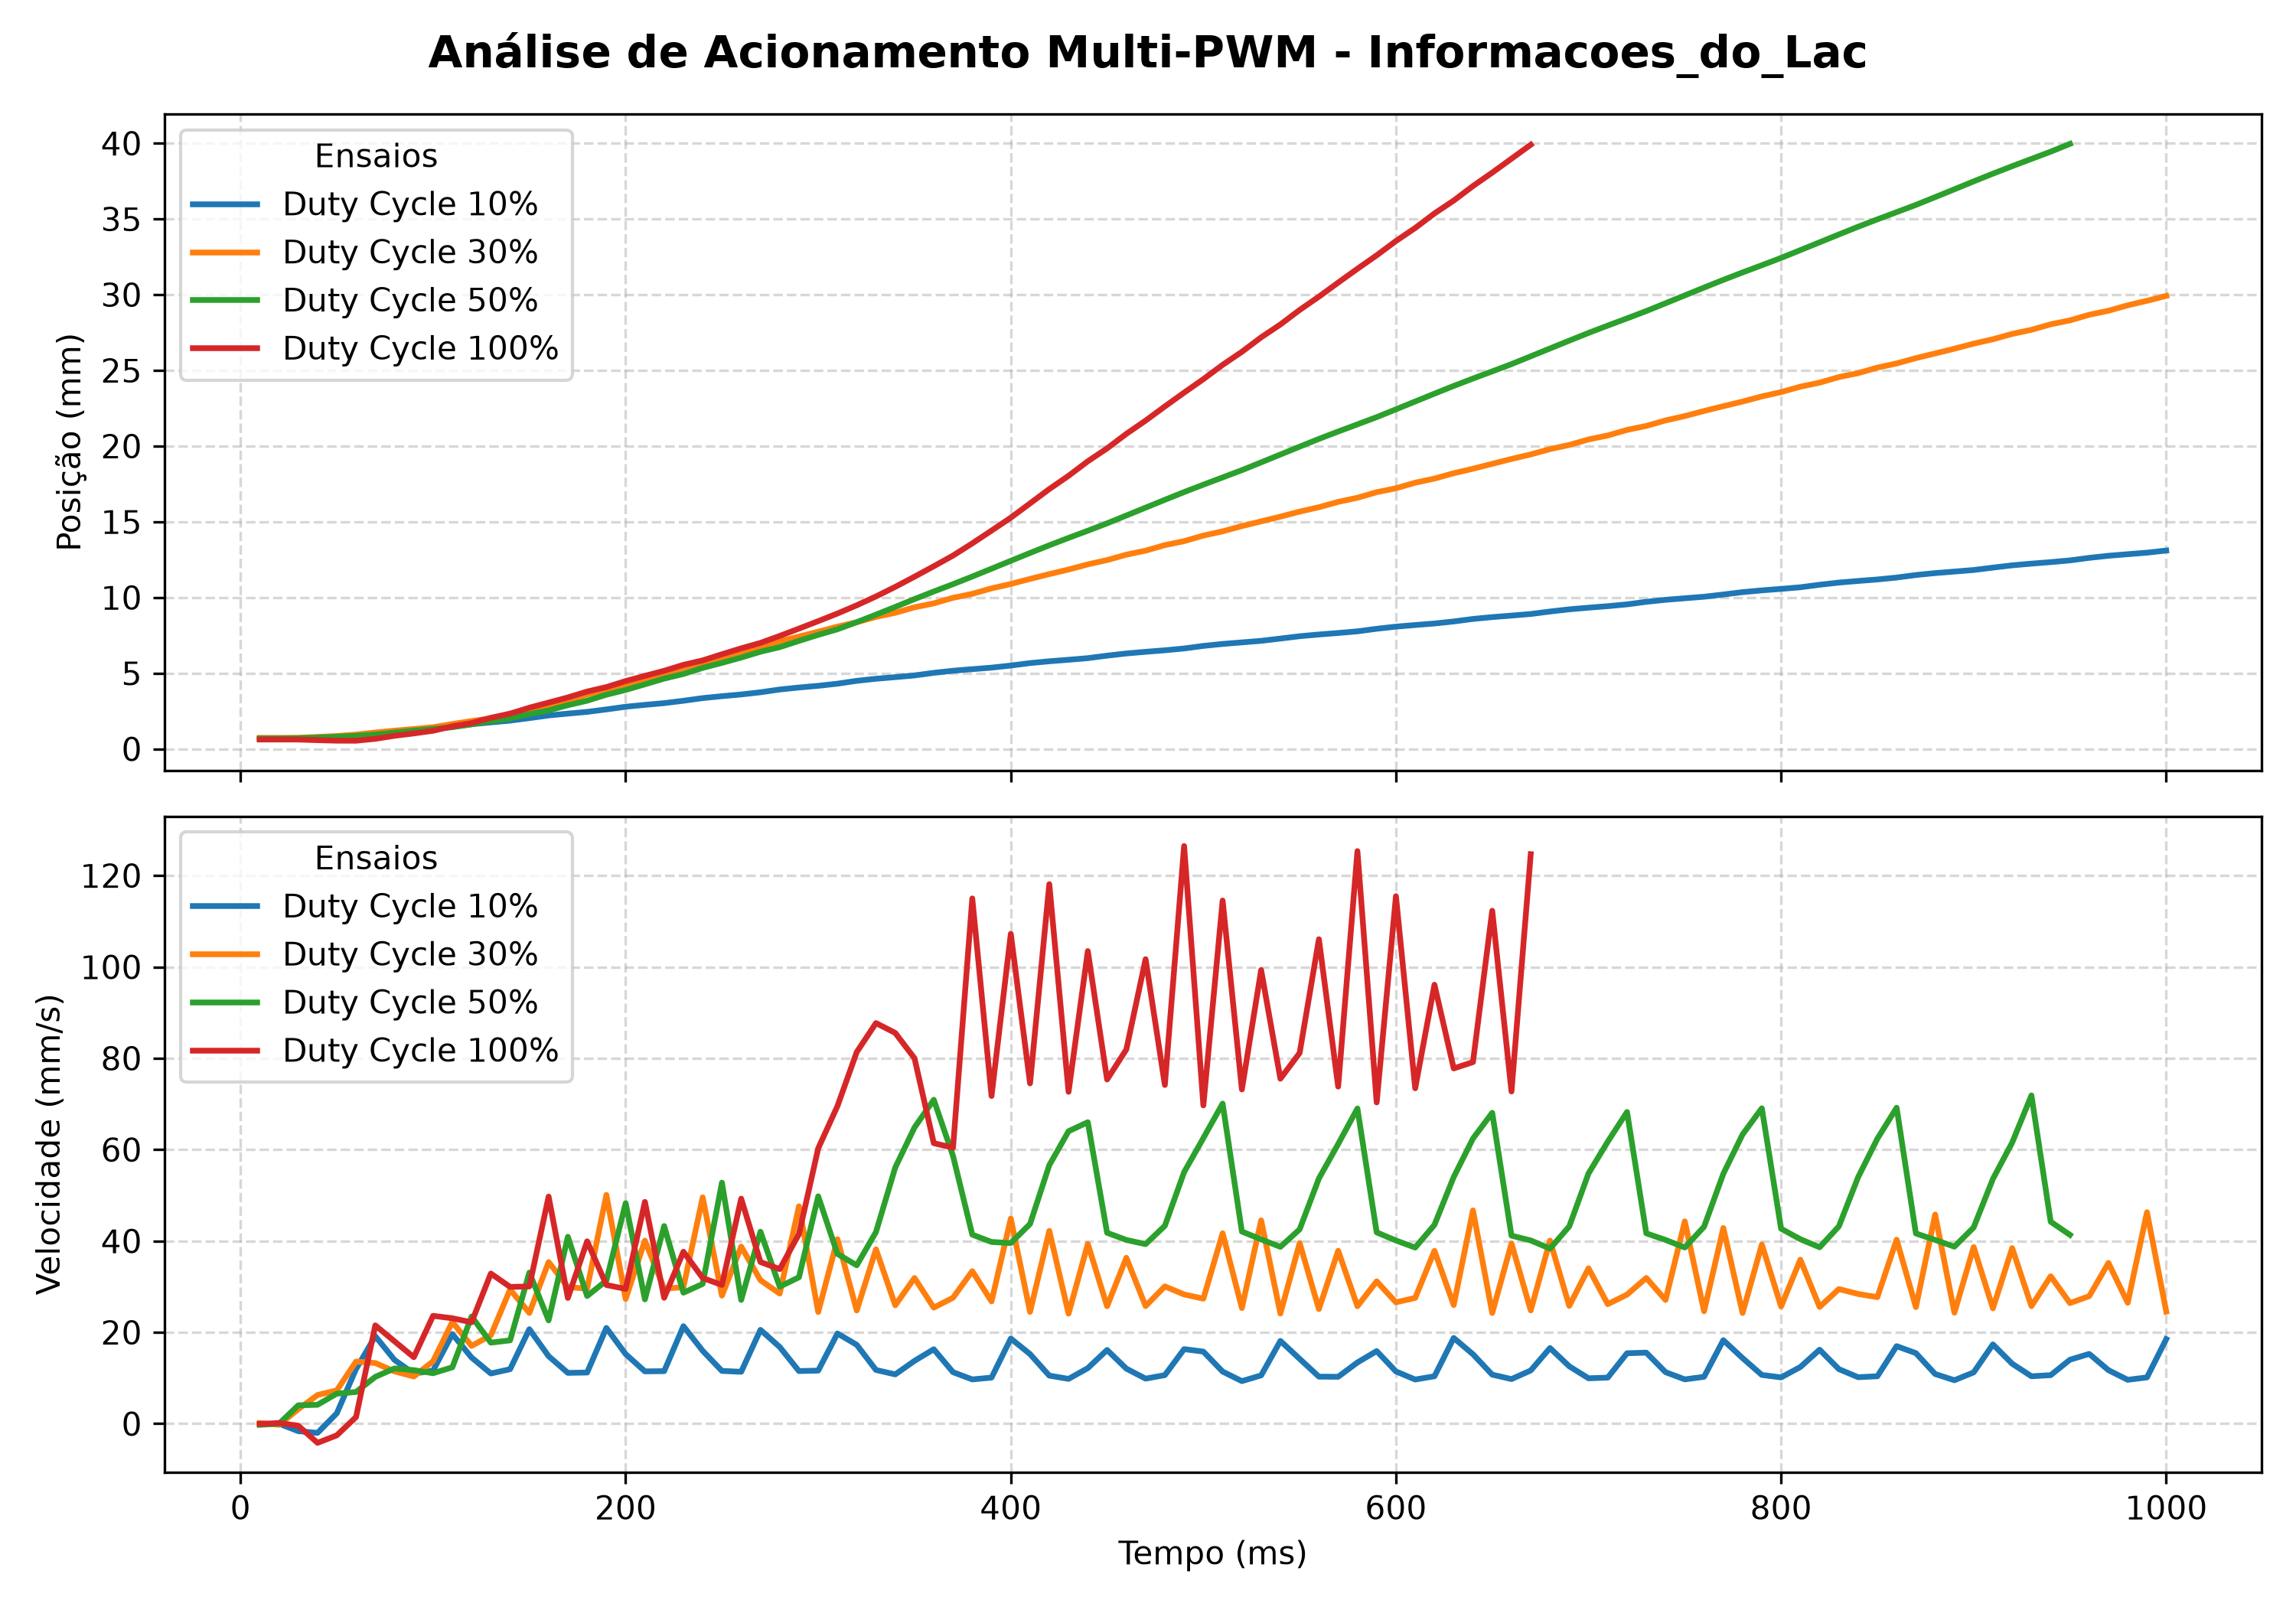
\includegraphics[width=0.8\textwidth]{figuras/grafico_multiduty_Informacoes_do_Lac_20261022_074203.png}
    \fonte{ O Autor.}
\end{figure}

Ao elevar o degrau para $30\%$,$50\%$ e $100\%$ de PWM, a velocidade linear máxima atingiu patamares transitórios de até $30\text{ mm/s}$ nas fases de final. Esses ensaios experimentais confirmaram que a resposta eletromecânica do atuador linear possui constante de tempo compatível com os requisitos de atuação rápida, respaldando a identificação da planta de primeira ordem para velocidade com ganho $K_{vel} = 1{,}306\text{ mm/s por \%PWM}$ e constante $\tau = 0{,}053\text{ s}$ utilizada no projeto do regulador LQI.
\par


\subsection{Identificação da relação posição--pressão}
\label{sec:resultado-final-plid}

Além do \texttt{OLTEST}, foram realizados três ensaios \texttt{PLID} para identificar a relação entre a posição do LAC e a pressão no circuito. O protocolo aplicou três níveis sucessivos, de 100, 200 e 300 psi, e registrou a fase de pressurização e o período de retenção. A Tabela~\ref{tab:resultado-final-plid} apresenta as médias obtidas durante a retenção. Os valores de pressão não devem ser interpretados como exatamente iguais ao alvo, pois a pressão continuou variando depois da transição para o modo \textit{hold}.

\begin{table}[htbp]
    \centering
    \caption{Resultados dos ensaios \texttt{PLID} durante a retenção.}
    \label{tab:resultado-final-plid}
    \begin{tabular}{c c c c c}
        \toprule
        Alvo (psi) & $P_{w,\mathrm{hold}}$ (psi) & $x_{\mathrm{hold}}$ (mm) & Faixa de $x_{\mathrm{hold}}$ (mm) & Ensaios \\
        \midrule
        100 & $106,4\pm0,6$ & $6,58\pm0,28$ & 6,41--6,92 & 3 \\
        200 & $216,9\pm2,0$ & $6,43\pm0,01$ & 6,40--6,44 & 3 \\
        300 & $312,4\pm4,4$ & $6,67\pm0,21$ & 6,50--6,90 & 3 \\
        \bottomrule
    \end{tabular}
    \Fonte{O autor, a partir dos ensaios \texttt{PLID}.}
\end{table}

Na fase de pressurização, os maiores valores registrados foram 94,13, 197,17 e 296,05 psi para os alvos de 100, 200 e 300 psi, respectivamente, no primeiro arquivo analisado. Assim, os alvos foram atingidos durante a retenção ou após a transição de fase. Esse comportamento evidencia a diferença entre a posição de cruzamento durante o movimento e a posição de equilíbrio durante o \textit{hold}, além de justificar a utilização de uma tabela de referência calibrada experimentalmente.

\begin{figure}[htbp]
    \centering
    \includegraphics[width=0.92\textwidth]{Matlab2/figuras/ensaio_plid_20260912_202531.png}
    \caption{Ensaio \texttt{PLID}: identificação dos transientes de pressão e da posição do LAC para os níveis de 100, 200 e 300 psi.}
    \label{fig:resultado-final-plid}
\end{figure}

O Código~\ref{cod:c-plid-retencao} mostra como o firmware detecta o cruzamento do nível de pressão de cada degrau, registra a posição correspondente e calcula as médias durante a retenção. Os dados enviados pelo firmware foram processados posteriormente para compor a Figura~\ref{fig:resultado-final-plid}.

\subsection{Tabela de referência entre 50 e 100 psi}
\label{sec:resultado-final-tabela-50-100}

Para organizar a faixa de menor pressão, foi utilizado o ponto do ensaio \texttt{STAIRCASE} mais próximo de 50 psi e o valor médio dos ensaios \texttt{PLID} na região de 100 psi. No ensaio \texttt{STAIRCASE} selecionado, a pressão média de 50,48 psi foi obtida com posição média de 5,88 mm. Para 100 psi, a posição média dos três ensaios \texttt{PLID} foi de aproximadamente 6,59 mm. Os pontos intermediários da Tabela~\ref{tab:resultado-final-referencia-50-100} são estimativas por interpolação linear entre esses dois resultados e não constituem medições diretas.

\begin{table}[htbp]
    \centering
    \caption{Referência de posição do LAC para a faixa de 50 a 100 psi.}
    \label{tab:resultado-final-referencia-50-100}
    \begin{tabular}{c c l}
        \toprule
        Pressão de referência (psi) & Posição do LAC (mm) & Origem do valor \\
        \midrule
        50 & 5,88 & Medição no \texttt{STAIRCASE}: 50,48 psi \\
        60 & 6,02 & Interpolação entre pontos medidos \\
        70 & 6,16 & Interpolação entre pontos medidos \\
        80 & 6,31 & Interpolação entre pontos medidos \\
        90 & 6,45 & Interpolação entre pontos medidos \\
        100 & 6,59 & Média dos três ensaios \texttt{PLID} \\
        \bottomrule
    \end{tabular}
    \Fonte{O autor. Os valores intermediários devem ser confirmados por ensaios específicos antes de serem usados como calibração definitiva.}
\end{table}

\begin{figure}[htbp]
    \centering
    \includegraphics[width=0.88\textwidth]{Matlab2/figuras/ensaio_staircase_curva_20260910_104748.png}
    \caption{Curva experimental de posição e pressão obtida no ensaio \texttt{STAIRCASE}.}
    \label{fig:resultado-final-staircase}
\end{figure}

No ensaio \texttt{STAIRCASE}, o firmware registra o alvo de posição, a posição medida e a pressão filtrada. Esse formato de aquisição, empregado no pós-processamento da curva, é apresentado no Código~\ref{cod:c-staircase-telemetria}.

\subsection{Estados funcionais das válvulas}
\label{sec:resultado-final-valvulas}

Os estados funcionais foram definidos no firmware por modos de acionamento do driver. A convenção elétrica adotada considera PFV e ORL normalmente fechadas e IRL e CSV normalmente abertas. A Tabela~\ref{tab:resultado-final-valvulas} apresenta os modos utilizados nos ensaios e deve ser interpretada como comando lógico, não como medição individual da corrente ou da tensão das solenóides.

\begin{table}[htbp]
    \centering
    \caption{Estados funcionais derivados para as válvulas do canal analisado.}
    \label{tab:resultado-final-valvulas}
    \begin{tabular}{l c c c c l}
        \toprule
        Modo funcional & PFV & IRL & ORL & CSV & Função hidráulica \\
        \midrule
        \texttt{Deenergized} & OFF & OFF & OFF & OFF & Estado sem acionamento \\
        \texttt{ApplyCandidate} & ON & ON & OFF & ON & Avanço do LAC e pressurização \\
        \texttt{HoldCandidate} & ON & OFF & OFF & ON & Retenção da pressão \\
        \texttt{ReleaseValidated} & OFF & OFF & ON & OFF & Alívio da pressão \\
        \bottomrule
    \end{tabular}
    \Fonte{Estados derivados pela função \texttt{deriveValveSignals} dos scripts de ensaio.}
\end{table}

A tabela representa estados comandados por software, e não quatro medições elétricas independentes. Nos arquivos de dados, os sinais disponíveis são principalmente os comandos agregados, o estado da máquina e, em alguns ensaios, o campo \texttt{valve\_mode}. Não foram registrados individualmente a corrente ou a tensão de cada solenóide.

No ensaio \texttt{PPMULTI}, foi utilizado tempo mínimo de permanência de 30 ms entre comandos de válvula, definido por \texttt{BRAKE\_PPMULTI\_VALVE\_MIN\_DWELL\_MS}. O \texttt{CLMULTI} inicialmente não possuía essa restrição e apresentou comutações rápidas entre aplicação e alívio, compatíveis com \textit{chattering} causado pela decisão a cada período de 1 ms. Esse resultado motivou a inclusão de uma temporização mínima no acionamento das válvulas.

\subsection{Condições de aquisição e estimativas de incerteza}
\label{sec:resultado-final-incerteza}

A aquisição do firmware foi configurada com período nominal de $1$ ms, enquanto o registro serial utilizado para inspeção foi realizado a cada aproximadamente $5$ ms. Para uma conversão ideal de uma faixa de 0--500 psi por um conversor de 12 bits, a resolução nominal seria de aproximadamente $0,122$ psi por contagem. Esse valor representa apenas a resolução da quantização e não a incerteza total da cadeia de medição. A Tabela~\ref{tab:resultado-final-aquisicao} reúne os valores disponíveis e identifica quais deles são estimativas de engenharia.

\begin{table}[htbp]
    \centering
    \caption{Condições de aquisição e estimativas utilizadas na interpretação dos ensaios.}
    \label{tab:resultado-final-aquisicao}
    \begin{tabular}{l l l}
        \toprule
        Parâmetro & Valor & Classificação \\
        \midrule
        Faixa nominal do sensor de pressão & 0--500 psi & Informação de projeto \\
        Resolução ideal de 12 bits & $0,122$ psi/LSB & Cálculo nominal \\
        Incerteza de pressão & $\pm5$ psi & Estimativa, não calibrada \\
        Resolução nominal de posição & aproximadamente $0,01$ mm & Informação de projeto \\
        Incerteza de posição & $\pm0,05$ mm & Estimativa mecânica \\
        Período do firmware & $1$ ms & Configuração nominal \\
        Registro serial & aproximadamente $5$ ms & Configuração de registro \\
        Temperatura do fluido & Não medida & Limitação experimental \\
        Pressão de suprimento & Não medida diretamente & Limitação experimental \\
        \bottomrule
    \end{tabular}
    \Fonte{O autor. As incertezas indicadas como estimativas não substituem uma calibração metrológica.}
\end{table}

Não foram instalados canais para temperatura do fluido ou para pressão de suprimento. Dessa forma, os ensaios foram realizados sob condições de laboratório, mas não permitem quantificar a influência térmica ou a variação da pressão de alimentação. A temperatura ambiente aproximada não deve ser apresentada como medição, pois não há registro instrumental associado aos arquivos analisados.

\subsection{Protocolo para repetição controlada}
\label{sec:resultado-final-protocolo-repeticao}

Com base na dispersão observada nos ensaios \texttt{PLID} e \texttt{CLMULTI}, foi definido um protocolo para os próximos ensaios de repetição. Cada corrida deve começar após a conclusão do procedimento \texttt{HOME}, com pressão próxima de zero e posição inicial registrada. O perfil de referência, os limites de segurança, a matriz de ganhos e o período de amostragem devem permanecer constantes em toda a bateria.

Para cada condição de referência, recomenda-se executar pelo menos cinco corridas válidas. Devem ser registrados o tempo desde o \texttt{HOME}, a tensão de alimentação, a temperatura ambiente quando disponível, a posição, a pressão, a referência, os comandos e o estado funcional das válvulas. Uma corrida deve ser descartada somente quando ocorrer falha de sensor, perda de comunicação, saturação prolongada, violação de limite mecânico ou outro critério definido antes da análise.

As métricas previstas são erro RMS, erro estacionário, sobressinal, tempo de subida entre 10\% e 90\%, posição média no \textit{hold}, pressão média no \textit{hold}, mediana, desvio padrão, intervalo interquartil e intervalo de confiança. Esse protocolo ainda é uma especificação de ensaio; ele não deve ser confundido com uma análise estatística já realizada.

Para uma bateria controlada, devem ser mantidos: posição inicial de aproximadamente $0,50\pm0,05$ mm, pressão inicial de $0\pm2$ psi, temperatura do fluido com variação inferior a $2$~$^{\circ}$C entre corridas, tensão de alimentação, ganhos do controlador e limites de segurança. O perfil recomendado é $0\rightarrow100\rightarrow200\rightarrow50\rightarrow0$ psi, com segmentos de 1 s. A bateria deve conter pelo menos cinco corridas válidas para cada configuração de \texttt{CLMULTI}, \texttt{PPMULTI}, \texttt{CLSTEP A} e \texttt{CLSTEP B}.

Quando a instrumentação estiver disponível, os sinais ambientais devem ser registrados no formato \texttt{[ENV],t\_ms,Tfluid\_C,Tamb\_C,Psup\_psi}. Os comandos elétricos individuais das válvulas podem ser registrados no formato \texttt{[VALVE],t\_ms,iPFV,iIRL,iORL,iCSV,vDriver}. Esses formatos são propostas de aquisição para os ensaios futuros e não correspondem a canais existentes nos CSVs analisados neste trabalho.

\section[Etapa I: resposta eletro-hidráulica ao degrau]{Etapa I: resposta eletro-hidráulica ao degrau}
\label{sec:resultado-final-clstep}

A Etapa I utiliza o ensaio auxiliar \texttt{CLSTEP B} para examinar a resposta eletro-hidráulica a uma referência em degrau, sob controle de posição do LAC. A implementação utilizada é descrita na Seção~\ref{sec:metodologia-procedimento} e no Código~\ref{cod:c-clstep-pi}. A referência de posição foi de aproximadamente $x_{\mathrm{ref}}=6{,}85$ mm, associada ao nível nominal de 100 psi pela curva posição--pressão. A pressão medida, a estimativa registrada, o erro de estimação, a posição e o esforço de controle permitem examinar o transiente e a retenção. A presença desses sinais no gráfico não implica equivalência entre essa implementação e o LQI com observador avaliado na Etapa II.

\begin{figure}[htbp]
    \centering
    \includegraphics[width=1.0\textwidth]{figuras/ensaio_clstepB_20260912_083523.png}
    \caption[Ensaio CLSTEP B: resposta eletro-hidráulica ao degrau.]{Etapa I -- Ensaio \texttt{CLSTEP B}: resposta eletro-hidráulica ao degrau sob controle de posição do LAC.}
    \label{fig:resultado-final-clstep}
\end{figure}

O tempo de subida entre 10\% e 90\% de 100 psi foi de 98 ms. A pressão máxima foi de aproximadamente 103,85 psi, correspondente a sobressinal de 3,8\%. A estabilização inicial ocorreu em aproximadamente 400 ms. Após esse intervalo, a pressão decaiu lentamente de cerca de 103 psi para aproximadamente 93 psi, produzindo erro estacionário de 7,14 psi em relação à referência de 100 psi.

A posição permaneceu próxima de $6{,}82$ mm durante o trecho de retenção. A diferença entre esse valor e a posição estimada para 100 psi, indicada no registro como aproximadamente $6{,}95$ mm, explica parte do erro observado. O decaimento lento também é compatível com relaxação viscoelástica das vedações e do fluido. Assim, o resultado positivo do ensaio está associado ao rápido alcance da região de pressão desejada e ao baixo sobressinal, enquanto a limitação aparece no erro residual durante a retenção.

\begin{table}[htbp]
    \centering
    \caption[Resultados do ensaio CLSTEP B.]{Resultados do ensaio auxiliar \texttt{CLSTEP B} na Etapa I.}
    \label{tab:resultado-final-clstep}
    \begin{tabular}{l l}
        \toprule
        Indicador & Resultado \\
        \midrule
        Referência de pressão & 100 psi \\
        Referência de posição & aproximadamente 6,85 mm \\
        Tempo de subida (10--90\%) & 98 ms \\
        Pressão máxima & 103,85 psi \\
        Sobressinal & 3,8\% \\
        Estabilização inicial & aproximadamente 400 ms \\
        Pressão no trecho final & aproximadamente 93 psi \\
        Erro estacionário & 7,14 psi \\
        \bottomrule
    \end{tabular}
    \Fonte{Dados registrados no ensaio \texttt{CLSTEP B}.}
\end{table}

O ensaio confirmou a viabilidade do mapeamento posição--pressão na condição específica da bancada. Entretanto, a relação $P_w=g(x)$ depende da compressibilidade do fluido, da presença de ar, da temperatura, da posição inicial, da histerese mecânica, das vedações e das condições do conjunto pastilha--disco--caliper. Portanto, a pressão estimada a partir do LAC precisa ser recalibrada quando essas condições forem alteradas. A medição de pressão disponível na bancada permanece necessária para validar a estimativa, embora não seja utilizada como entrada do controlador de posição.

\subsection{Curva preliminar de calibração}
\label{sec:resultado-final-lut}

A combinação dos ensaios \texttt{STAIRCASE} e \texttt{PLID} permite organizar uma curva experimental para a conversão de pressão em posição nas condições avaliadas. A Tabela~\ref{tab:resultado-final-lut} reúne os pontos utilizados no controle: os pontos de baixa pressão foram obtidos no \texttt{STAIRCASE}, os pontos de maior pressão foram obtidos ou aproximados a partir do \texttt{PLID}, e alguns valores são interpolados ou extrapolados.

\begin{table}[htbp]
    \centering
    \caption{Pontos da curva experimental $P_w=g(x)$ e origem dos valores.}
    \label{tab:resultado-final-lut}
    \begin{tabular}{c c l}
        \toprule
        Posição $x$ (mm) & Pressão $P_w$ (psi) & Origem \\
        \midrule
        0,90 & 0,0 & Medição no \texttt{STAIRCASE} \\
        1,40 & 0,0 & Medição no \texttt{STAIRCASE}; região de curso morto \\
        1,90 & 0,7 & Medição no \texttt{STAIRCASE} \\
        2,40 & 2,5 & Medição no \texttt{STAIRCASE} \\
        3,20 & 6,7 & Medição no \texttt{STAIRCASE} \\
        3,90 & 11,8 & Medição no \texttt{STAIRCASE} \\
        4,30 & 17,2 & Medição no \texttt{STAIRCASE} \\
        4,90 & 24,9 & Medição no \texttt{STAIRCASE} \\
        5,40 & 35,0 & Interpolação \\
        5,90 & 50,0 & Aproximação no \texttt{STAIRCASE} \\
        6,40 & 70,0 & Interpolação entre pontos do \texttt{PLID} \\
        6,91 & 107,0 & Aproximação no \texttt{PLID} \\
        7,10 & 180,0 & Estimativa a partir do cruzamento \\
        7,25 & 250,0 & Estimativa a partir do cruzamento \\
        7,35 & 316,0 & Extrapolação \\
        \bottomrule
    \end{tabular}
    \Fonte{O autor. A curva foi identificada para as condições de ensaio documentadas.}
\end{table}

Os dados indicam uma região de curso morto até aproximadamente $1,4$ mm, seguida de crescimento gradual até cerca de 50 psi e de uma região mais inclinada acima de aproximadamente $5,9$ mm. A inclinação aparente nessa região não deve ser tratada como constante, pois os dados de retenção e cruzamento apresentam trajetórias diferentes.

Os ensaios \texttt{PLID} fornecem uma evidência indireta dessa dependência. Nos níveis de 100, 200 e 300 psi, as diferenças entre as posições de cruzamento e de retenção foram aproximadamente $0,12$, $0,51$ e $0,55$ mm, respectivamente, considerando os valores médios dos ensaios. Essa diferença não constitui, por si só, uma curva de descida, mas mostra que a posição do LAC não determina univocamente a pressão sem considerar a trajetória e o tempo de retenção.

\subsection{Histerese da relação posição--pressão}
\label{sec:resultado-final-histerese}

Os dados disponíveis permitem identificar a influência da trajetória, mas não quantificam integralmente a histerese. Para completar essa caracterização, deve-se aplicar uma sequência \texttt{STAIRCASE} de subida e descida, com incrementos de aproximadamente $0,25$ mm entre $0,9$ e $7,3$ mm. Cada patamar deve permanecer em retenção por pelo menos $1,5$ s, permitindo calcular a posição média, a pressão média e o desvio durante o patamar.

As curvas de subida e descida devem ser processadas separadamente. Recomenda-se realizar três ciclos completos, ida e volta, mantendo os mesmos patamares. A diferença
\begin{equation}
    \Delta P_{w,\mathrm{hist}}(x) = P_{w,\mathrm{descida}}(x) - P_{w,\mathrm{subida}}(x)
\end{equation}
quantifica a histerese em pressão em cada posição. A área entre as curvas pode ser calculada por integração numérica. O ensaio também deve registrar o deslocamento durante o \textit{hold}, pois a variação lenta observada no \texttt{CLSTEP B} pode alterar a posição equivalente à pressão de referência. Os dados atualmente disponíveis não contêm as três repetições bidirecionais completas; portanto, esses valores ainda não são resultados deste trabalho.

\begin{figure}[htbp]
    \centering
    \includegraphics[width=0.92\textwidth]{Matlab2/figuras/ensaio_clstepA_20260912_082531.png}
    \caption{Ensaio \texttt{CLSTEP A}, com realimentação direta da pressão, utilizado como referência experimental.}
    \label{fig:resultado-final-clstep-a}
\end{figure}

\begin{figure}[htbp]
    \centering
    \includegraphics[width=0.92\textwidth]{figuras/ensaio_clstepB_20260912_083523.png}
    \caption[Ensaio CLSTEP B: posição do LAC e pressão registrada.]{Ensaio auxiliar \texttt{CLSTEP B} da Etapa I, com controle de posição do LAC e registro da pressão resultante.}
    \label{fig:resultado-final-clstep-b}
\end{figure}

\section[Etapa II: avaliação do LQI e ensaios complementares]{Etapa II: avaliação do LQI e ensaios complementares}
\label{sec:resultado-final-complementares}

A Etapa II concentra a avaliação embarcada do LQI com observador de Luenberger nos ensaios de múltiplas referências. Enquanto a Etapa I examina a resposta a um degrau em uma configuração auxiliar, esta etapa analisa o seguimento de referências e a pressão produzida nas configurações LQI documentadas. Os indicadores do \texttt{CLSTEP B} permanecem restritos à Etapa I e não são utilizados como medidas de desempenho do LQI. O perfil \texttt{CLMULTI} aplica a sequência $0\rightarrow100\rightarrow200\rightarrow50\rightarrow0$ psi; o modelo discreto, o observador e a lei LQI embarcada estão no Código~\ref{cod:c-clmulti-lqi}. No \texttt{PPMULTI}, a malha interna emprega LQR com ação integral para controlar a posição, enquanto a malha externa corrige a referência de posição a partir do erro de pressão. O modelo discreto, o observador e a lei de controle estão no Código~\ref{cod:c-ppmulti-lqi}; o formato dos dados enviados para geração da Figura~\ref{fig:resultado-final-ppmulti} está no Código~\ref{cod:c-ppmulti-telemetria}. O \texttt{PWMSWEEP} fornece dados para a identificação da dinâmica do LAC.

\begin{figure}[htbp]
    \centering
    \includegraphics[width=0.92\textwidth]{figuras/ensaio_clmulti_20260912_091937.png}
    \caption{Ensaio \texttt{CLMULTI} com múltiplos patamares de referência.}
    \label{fig:resultado-final-clmulti}
\end{figure}

O ensaio  \texttt{CLMULTI} (Figura~\ref{fig:resultado-final-clmulti}), percorreu a sequência $0\rightarrow100\rightarrow200\rightarrow50\rightarrow0$ psi, com transições em 1, 2, 3 e 4~s. O registro de 1~kHz disponível cobre o intervalo de 0 a 4,999~s, incluindo a despressurização final. No patamar nominal de 100~psi, a pressão máxima foi de 94,74~psi e a média do segmento foi de 65,52~psi. Essa média inclui o transiente inicial; nos últimos 51 registros do segmento, a pressão média foi de aproximadamente 89,25~psi. No patamar de 200~psi, o pico foi de 185,90~psi e a média do segmento foi de 166,16~psi. O deslocamento do LAC situou-se aproximadamente entre 7,1 e 7,5~mm nessa etapa.

Na transição para 50~psi, a pressão apresentou um transiente de alívio e aproximou-se da referência, com erro final absoluto de 1,07~psi. Após a referência retornar a zero, o circuito foi despressurizado até valores próximos de zero no registro. A execução de todas as transições demonstra a operação da sequência de pressurização e alívio, mas os desvios de 10,75 e 29,08~psi ao final dos patamares de 100 e 200~psi não são desprezíveis. A calibração posição--pressão pode contribuir para esses desvios, sem que o ensaio isole sua causa. A estimativa de pressão também apresenta oscilações no patamar de 200~psi e permanece afastada da medição após o alívio.

\begin{figure}[htbp]
    \centering
    \includegraphics[width=0.92\textwidth]{figuras/ensaio_ppmulti_20260916_083850.png}
    \caption{Ensaio \texttt{PPMULTI}: referência, contribuições das malhas de controle, posição do LAC e pressão medida.}
    \label{fig:resultado-final-ppmulti}
\end{figure}

O ensaio \texttt{PPMULTI} (Figura~\ref{fig:resultado-final-ppmulti}) avalia a resposta dinâmica da arquitetura em malha dupla, na qual a malha interna do regulador LQI controla o posicionamento do atuador linear e a malha externa corrige a referência com base no erro de pressão medido. O gráfico temporal demonstra a convergência coordenada entre as ações de controle: o termo de posição ($u_{pos}$) assegura o avanço rápido para transposição da folga inicial mecânica, enquanto o termo de pressão ($u_{pw}$) atua atenuando gradualmente os desvios decorrentes da complacência do circuito.

O sistema percorre a sequência de referências estabelecida, registrando tempos de resposta compatíveis com a modulação ativa de freio. No degrau de 100 psi, observa-se rápida pressurização com amortecimento transitório progressivo; no patamar de 200 psi, a atuação coordenada permite atingir níveis elevados de pressão sem ocorrência de instabilidades. Nas transições de alívio para 50 psi e retorno a 0 psi, a malha externa atua em conjunto com a lógica de comando das válvulas, garantindo despressurização suave e controlada. Os leves sobre-sinais e as ondulações transitórias registradas nas comutações de patamar refletem a dinâmica de acomodação viscoelástica do fluido e o tempo de chaveamento dos drivers, confirmando a viabilidade da estratégia em cascata para atenuar as não linearidades hidráulicas na bancada.

\begin{table}[htbp] 
    \centering 
    \caption{Métricas de desempenho observadas no ensaio de controle indireto \texttt{CLMULTI}.}
    \label{tab:resultado-final-clmulti-metricas} 
    \begin{tabular}{l c c c c c} 
        \toprule 
        Segmento & $P_{\mathrm{ref}}$ (psi) & $e_{\mathrm{RMS}}$ (psi) & $e_{\mathrm{SS}}$ (psi) & $\overline{P}w$ (psi) & $P{w,\max}$ (psi) \\ 
        \midrule 
        Patamar 1 & 100 & 51,81 & 10,75 & 65,52 & 94,74 \\ 
        Patamar 2 & 200 & 41,98 & 29,08 & 166,16 & 185,90 \\ 
        Descida & 50 & 20,17 & 1,07 & 54,17 & 170,84 \\ 
        Alívio & 0 & 12,68 & 0,00 & 6,01 & 51,18 \\ 
        \bottomrule 
    \end{tabular} 
    \Fonte{O autor, a partir dos registros de ensaio em bancada experimental.} 
\end{table}

A Tabela~\ref{tab:resultado-final-clmulti-metricas} refere-se exclusivamente ao \texttt{CLMULTI} da Figura~\ref{fig:resultado-final-clmulti}. Para cada segmento de 1~s, $e_{\mathrm{RMS}}$ considera todas as amostras, $e_{\mathrm{SS}}$ é o módulo da diferença entre a referência e a média das últimas 51 amostras, e $\overline{P}_w$ é a média de todo o segmento. Nos segmentos descendentes, o máximo inclui a pressão herdada do patamar anterior e não deve ser interpretado como sobressinal de pressurização. A leitura conjunta dos ensaios documenta a execução das transições, mantendo separadas a avaliação quantitativa do \texttt{CLMULTI} e a análise gráfica da nova configuração em cascata.

\begin{figure}[htbp]
    \centering
    \includegraphics[width=0.92\textwidth]{Matlab2/figuras/ensaio_pwmsweep_curvas_20260910_110520.png}
    \caption{Varredura de PWM utilizada para observar a resposta de posição e pressão do atuador linear.}
    \label{fig:resultado-final-pwmsweep}
\end{figure}

Os arquivos \texttt{PWMSWEEP} já estão organizados para estimar a constante de tempo $\tau$ e o ganho de velocidade $K_{\mathrm{vel}}$. A figura é apresentada como evidência do procedimento de identificação, enquanto os valores finais dependem da execução uniforme do script \texttt{identify\_tau\_gain\_from\_csv.m} em todos os arquivos válidos.

Para a identificação, considera-se inicialmente o modelo de primeira ordem
\begin{equation}
    \frac{v_{\mathrm{LAC}}(s)}{u(s)} = \frac{K_{\mathrm{vel}}}{\tau s+1},
\end{equation}
em que $u$ é o percentual de PWM e $v_{\mathrm{LAC}}$ é a velocidade do atuador. Para cada janela de PWM aproximadamente constante, $K_{\mathrm{vel}}$ pode ser calculado pela razão entre a velocidade média de regime e o PWM aplicado. A constante $\tau$ pode ser obtida pelo instante em que a velocidade alcança 63,2\% do valor final ou por ajuste exponencial do transiente.

Os arquivos \texttt{PWMSWEEP} disponíveis incluem comandos de 8\%, 15\%, 25\%, 50\%, 75\% e 100\% de PWM. Para a configuração adotada no controlador, foram utilizados $\tau=0,053$ s e $K_{\mathrm{vel}}=1,306$ mm/s por \%PWM. Esses parâmetros foram empregados na discretização e apresentaram resposta compatível com o comportamento observado do atuador nas condições avaliadas. O cálculo considera $K_{\mathrm{vel}}=v_{\mathrm{regime}}/u$ e a constante de tempo associada ao instante em que a velocidade alcança 63,2\% de $v_{\mathrm{regime}}$.

Com $T_s=1$ ms, a discretização ZOH utilizada no observador e no controlador foi registrada por
\begin{equation}
    \Phi = \begin{bmatrix}
        1 & 0{,}000990625092 \\
        0 & 0{,}981308960528
    \end{bmatrix}, \qquad
    \Gamma = \begin{bmatrix}
        0{,}000012243629833 \\
        0{,}024410497550323
    \end{bmatrix}.
\end{equation}
Esses valores são compatíveis com $\Phi_{22}=e^{-T_s/\tau}$ e $\Gamma_2=K_{\mathrm{vel}}(1-\Phi_{22})$ para os parâmetros de trabalho adotados. A verificação analítica confirma a coerência interna do modelo discretizado, mas não substitui a identificação experimental final.

\subsection{Repetibilidade dos ensaios}
\label{sec:resultado-final-repetibilidade}

Os três ensaios \texttt{PLID} permitem uma análise preliminar de repetibilidade. Para os níveis de 100, 200 e 300 psi, foram calculadas médias e desvios padrão das posições e pressões registradas. Os resultados são apresentados na Tabela~\ref{tab:resultado-final-repetibilidade-plid}.

\begin{table}[htbp]
    \centering
    \caption{Repetibilidade preliminar dos ensaios \texttt{PLID}.}
    \label{tab:resultado-final-repetibilidade-plid}
    \begin{tabular}{l c c}
        \toprule
        Grandeza & Média & Desvio padrão \\
        \midrule
        $x_{\mathrm{cruz}}$ em 100 psi & 6,70 mm & 0,28 mm \\
        $P_{w,\mathrm{hold}}$ em 100 psi & 106,4 psi & 0,6 psi \\
        $x_{\mathrm{hold}}$ em 100 psi & 6,58 mm & 0,28 mm \\
        $x_{\mathrm{cruz}}$ em 200 psi & 6,94 mm & 0,03 mm \\
        $P_{w,\mathrm{hold}}$ em 200 psi & 216,9 psi & 2,0 psi \\
        $x_{\mathrm{hold}}$ em 200 psi & 6,43 mm & 0,01 mm \\
        $x_{\mathrm{cruz}}$ em 300 psi & 7,22 mm & 0,11 mm \\
        $P_{w,\mathrm{hold}}$ em 300 psi & 312,4 psi & 4,4 psi \\
        $x_{\mathrm{hold}}$ em 300 psi & 6,67 mm & 0,21 mm \\
        \bottomrule
    \end{tabular}
    \Fonte{O autor, a partir das três repetições \texttt{PLID}.}
\end{table}

\subsection{Limites da comparação entre os ensaios CLSTEP A e B}
\label{sec:resultado-final-comparacao-clstep}

Os ensaios \texttt{CLSTEP A} e \texttt{CLSTEP B} avaliaram configurações distintas. No modo A, a pressão medida participa da realimentação; no modo B, o firmware fornecido fecha a malha na posição do LAC, e a pressão é registrada para caracterizar a resposta hidráulica. A comparação entre os modos requer condições iniciais, perfis de referência e critérios de avaliação equivalentes.

Os arquivos de aquisição de 1~kHz disponíveis compreendem oito corridas \texttt{CLSTEP A} e dez corridas \texttt{CLSTEP B}. No modo A, três corridas não apresentam elevação mensurável de pressão, duas atingem máximos de apenas 64,18 e 69,39 psi, e três ultrapassam 100 psi, incluindo dois picos próximos de 244--248 psi. No modo B, três corridas não alcançam 90 psi; as demais apresentam máximos entre aproximadamente 91,6 e 175 psi. Essa dispersão, somada à ausência de metadados suficientes para confirmar a equivalência de parâmetros e condições entre todas as aquisições, impede definir com rigor um conjunto homogêneo de corridas válidas. Por esse motivo, não se apresentam medianas ou intervalos interquartis agregados, nem se conclui que um modo seja estatisticamente superior ao outro. O ensaio \texttt{CLSTEP B} é discutido individualmente na Tabela~\ref{tab:resultado-final-clstep}; seus indicadores não representam a distribuição de todas as corridas.

No conjunto \texttt{CLMULTI}, quatro ensaios representativos no degrau de 100 psi apresentaram erro RMS médio de 56,26 psi, erro estacionário médio de 27,14 psi, sobressinal médio de 31,4\% e pressão máxima média de 131,39 psi. Os desvios padrão foram, respectivamente, 9,73 psi, 27,93 psi, 34,5\% e 34,41 psi. A dispersão elevada indica que o ajuste utilizado não produziu desempenho repetível nas condições avaliadas. Como os ganhos e as condições de execução não foram mantidos integralmente constantes, esses valores são usados como diagnóstico de desenvolvimento, e não como validação estatística definitiva.

\begin{table}[htbp]
    \centering
    \caption{Dispersão observada no degrau de 100 psi dos ensaios \texttt{CLMULTI}.}
    \label{tab:resultado-final-clmulti-repetibilidade}
    \begin{tabular}{l c c c c}
        \toprule
        Ensaio & $e_{\mathrm{RMS}}$ (psi) & $e_{\mathrm{SS}}$ (psi) & $M_p$ (\%) & $P_{w,\max}$ (psi) \\
        \midrule
        Ensaio 1 & 49,57 & 4,15 & 2,3 & 102,33 \\
        Ensaio 2 & 70,59 & 63,60 & 77,3 & 177,28 \\
        Ensaio 3 & 54,27 & 36,08 & 40,7 & 140,71 \\
        Ensaio 4 & 50,60 & 4,72 & 5,2 & 105,22 \\
        \midrule
        Média & 56,26 & 27,14 & 31,4 & 131,39 \\
        Desvio padrão & 9,73 & 27,93 & 34,5 & 34,41 \\
        \bottomrule
    \end{tabular}
    \Fonte{O autor, a partir dos ensaios \texttt{CLMULTI} selecionados.}
\end{table}

\section{Síntese dos resultados e limitações experimentais}
\label{sec:resultado-final-sintese}

Os resultados articulam a avaliação computacional e os ensaios experimentais. Nas simulações, o LQI com observador de Luenberger acompanhou referências de pressão no modelo hidráulico de duas pressões. Na bancada, os ensaios iniciais mostraram que a bomba centrífuga não estabelecia a pressão requerida e recirculava o fluido, o que levou à sua substituição pelo LAC. Os ensaios com LQI embarcado avaliaram o controle da posição do atuador e a pressão hidráulica resultante.

A integração também mostrou que a comunicação USB com o computador hospedeiro não atendia aos requisitos temporais observados, motivando a execução embarcada dos controladores no AURIX TC375. Os ensaios \texttt{PLID} e \texttt{STAIRCASE} permitiram caracterizar a relação posição--pressão. Na Etapa I, o ensaio auxiliar \texttt{CLSTEP B} apresentou pressão máxima de 103,85 psi, sobressinal de 3,8\% para o nível nominal de 100 psi e tempo de subida de 98 ms. A pressão decaiu para aproximadamente 93 psi durante a retenção, evidenciando a necessidade de avaliar a resposta hidráulica além do posicionamento. Na Etapa II, o LQI foi avaliado nos ensaios de múltiplas referências, que apresentaram dispersão e desvios relevantes. Portanto, os dados demonstram a execução e a avaliação experimental dos controladores, mas não comprovam atendimento a requisitos veiculares.

O sensor de pressão integrado ao bloco hidráulico utiliza uma interface serial compatível com a família de protocolos OSPI descrita em documentação de fabricantes de circuitos integrados. Entretanto, a implementação específica do sensor e do módulo não estava disponível para leitura direta pelo sistema desenvolvido, pois os detalhes de acesso dependiam de informações proprietárias dos fornecedores. Por essa razão, a interface não foi utilizada na arquitetura de controle. A pressão foi estimada indiretamente a partir da posição do LAC e o sensor disponível foi mantido para monitoramento e validação.
